\documentclass{article}
\usepackage{amsmath}
\usepackage{amssymb}
\usepackage{graphicx}
\usepackage{hyperref}
\usepackage[version=4]{mhchem}


\begin{document}
Show that The angle bisector of a triangle divides the opposite side into segments that are proportional to the adjacent sides.

\[
\frac{A B}{A C}=\frac{B D}{C D} \quad \text { or } \quad \frac{A B}{B D}=\frac{A C}{C D}
\]

Proof:
\begin{center}
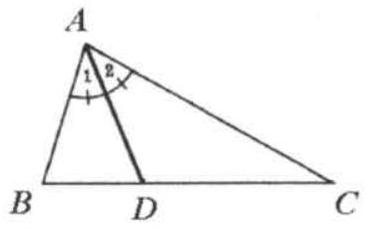
\includegraphics[width=\textwidth]{images/075.jpg}
\end{center}

Draw \(A H \perp B C\) at \(H\). The ratio of the areas \(\triangle A B D\) and

\[
A D C \text { is } \frac{S_{\triangle A B D}}{S_{\triangle A D C}}=\frac{\frac{1}{2} B D \times A H}{\frac{1}{2} C D \times A H}=\frac{B D}{C D} .
\]

Draw \(D E \perp A B, D F \perp A C\).\\
By Theorem 3.2, \(D E=D F\).\\
The ratio of the areas \(\triangle A B D\) and \(A D C\) is\\
We also know that \(\frac{S_{\triangle A B D}}{S_{\triangle A D C}}=\frac{\frac{1}{2} A B \times D E}{\frac{1}{2} A C \times D F}=\frac{A B}{A C}\)\\
\centering
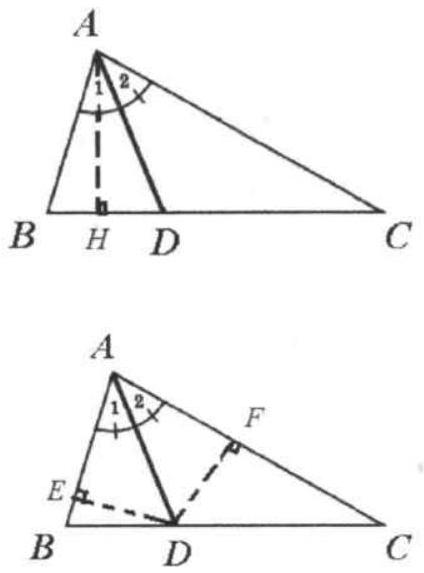
\includegraphics[width=\textwidth]{images/075(2).jpg}


Therefore: \(\frac{A B}{A C}=\frac{B D}{C D}\).


\end{document}
